\chapter{Modeling of Train Operations}
\label{chap:ModelingOfTrainOperations}
\par\noindent
\emph{\textbf{Introduction}} As has been noted in \ref{sec:Solution}, it is necessary to model the braking process of freight trains. All modeling work has been performed with Matlab Simulink. 

\section{Initial Model}
\label{sec:InitialModel}
\par\noindent
The initial model to be expanded upon describes a single braking process. It's sole input, apart from some constants, is pressure over time, meaning a distinct value ranging between 5 and 3.5 bar for every timestamp. For visualization, please refer to \ref{fig:initmodel_siminput}. Let's take a look at the whole model first. 

\begin{figure}[H]
	\centering
	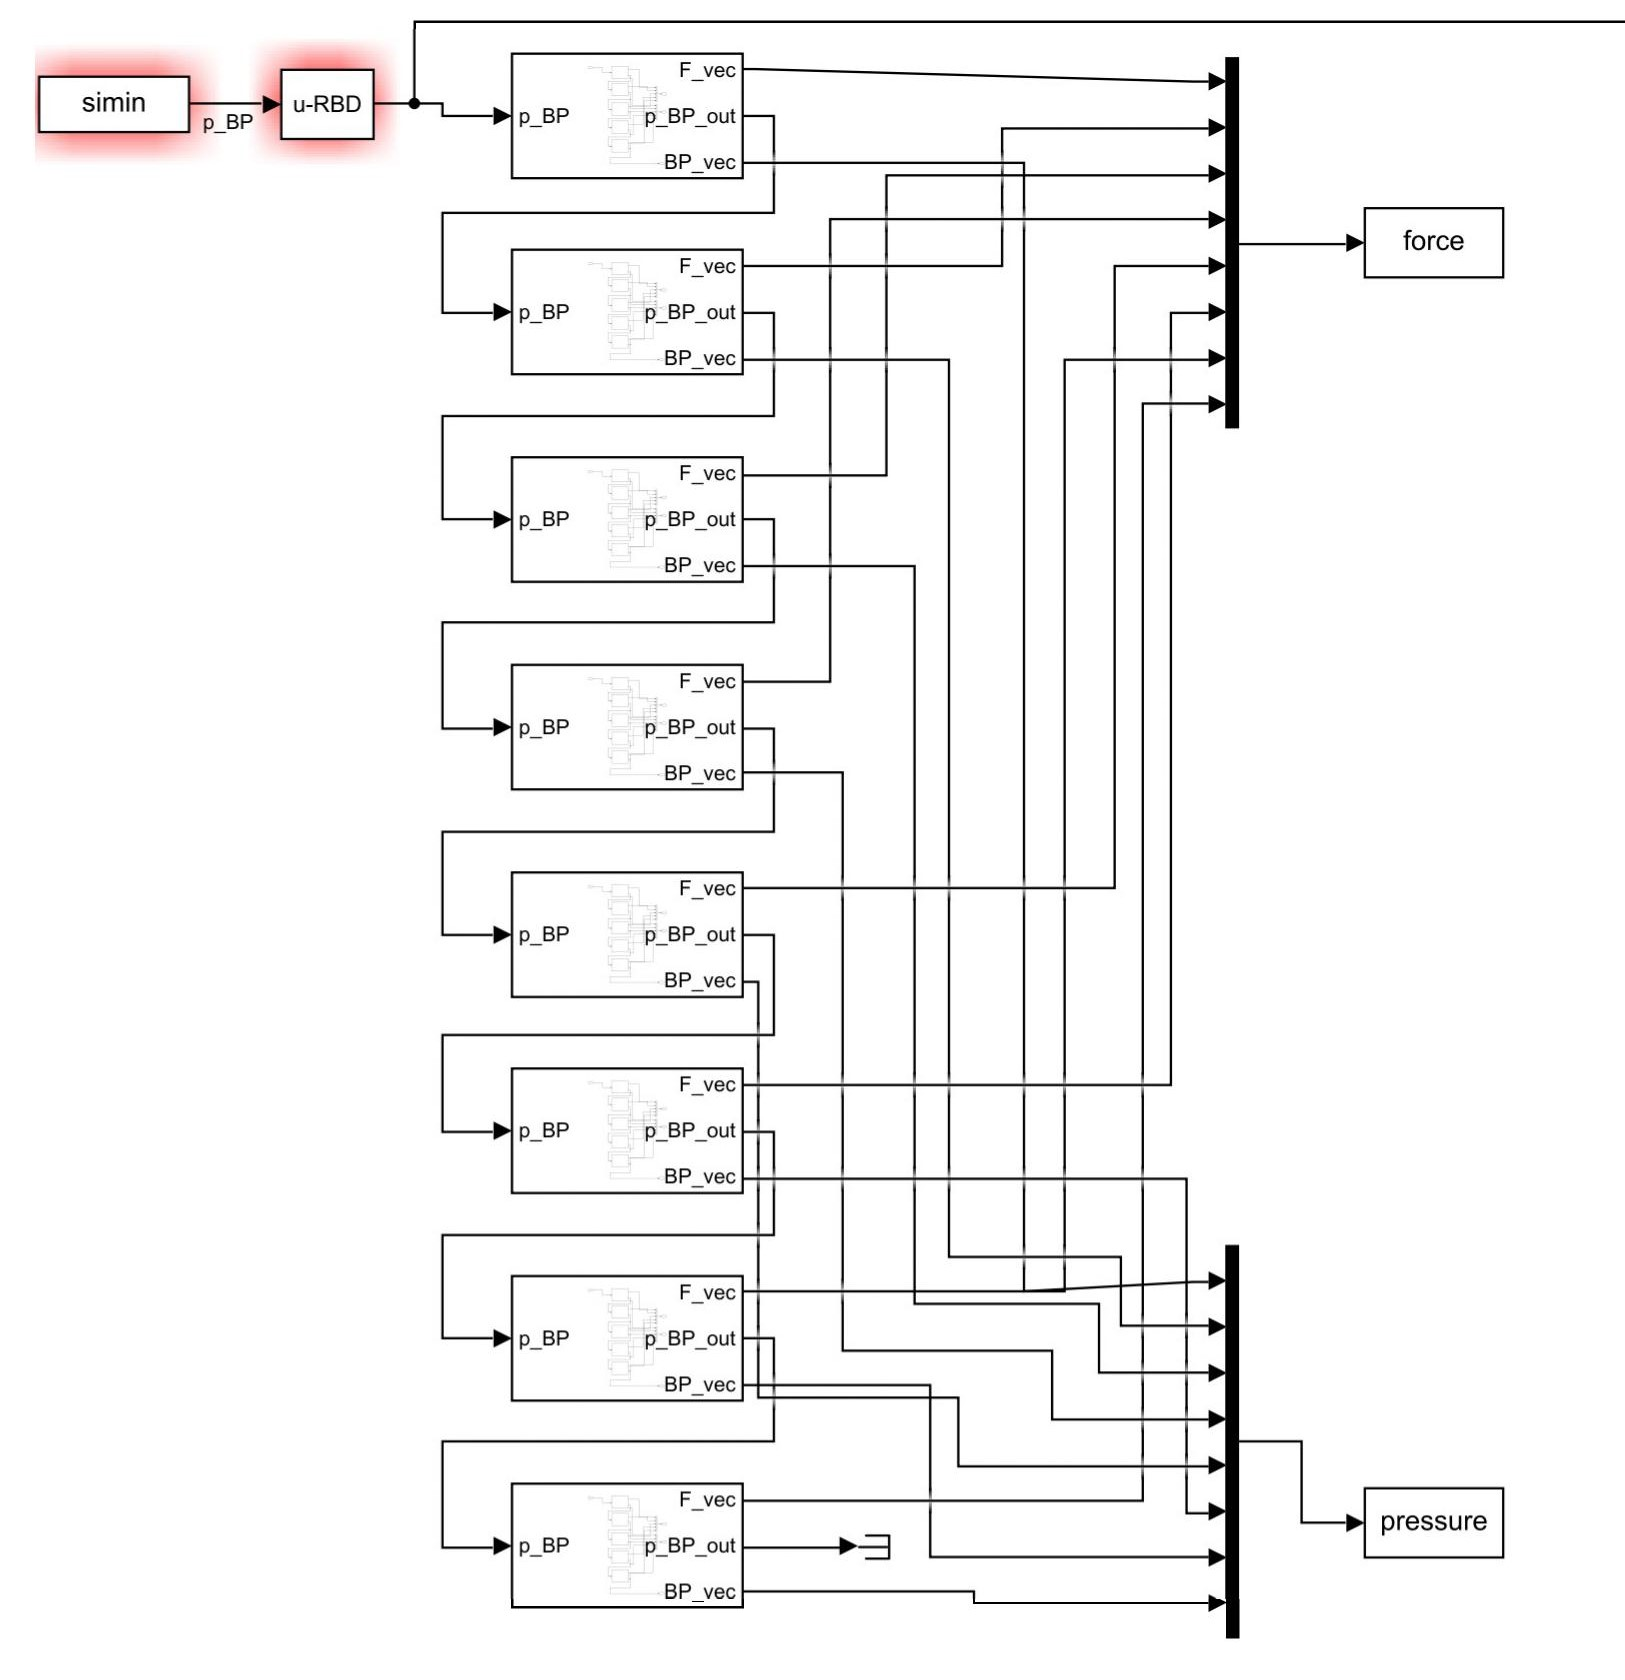
\includegraphics[width=\linewidth]{./pic/initmodel_whole}
	\caption{Initial Model}
	\label{fig:initmodel_whole}
\end{figure}

\par\noindent
Here we see a model of a freight train of fixed length, consisting of 40 wagons, which are, for better readability, further condensed to subsystems of five wagons each, so there are eight of these subsystems. They are interconnected via braking pipe, which is also the sole input to each system. Outputs are braking pressure and braking force. We will take a look at the actual wagon model next.

\begin{figure}[H]
	\centering
	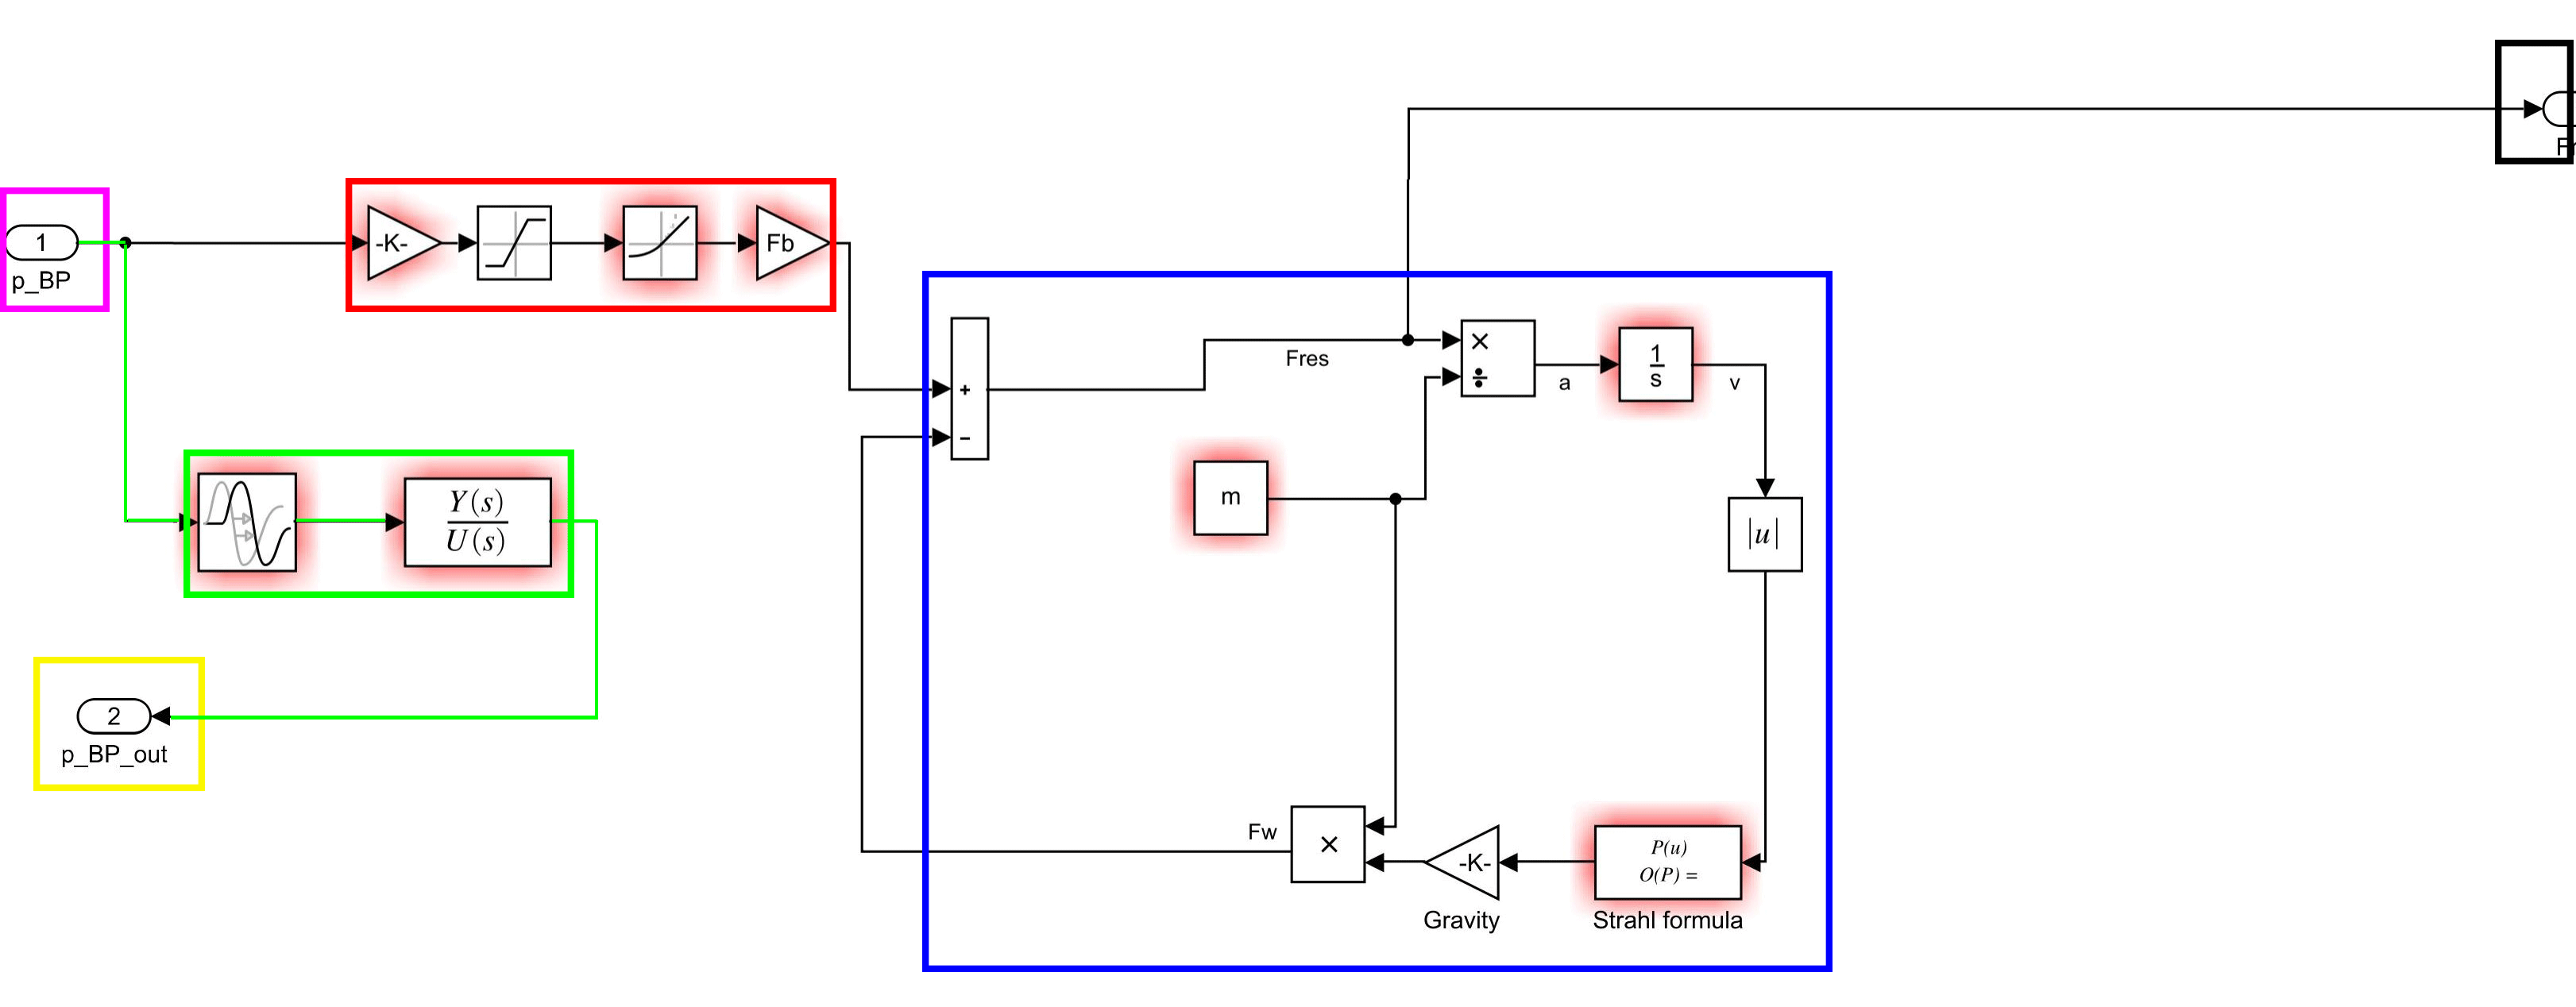
\includegraphics[width=\linewidth]{./pic/initmodel_wagon}
	\caption{Initial Model - Wagon}
	\label{fig:initmodel_wagon}
\end{figure}

\par\noindent
Above is the initial wagon model. \NOTE{All 40 wagon models are identical here. This will be addressed in section \ref{sec:ModelExpansion}}. It consists of three main components.
\par
In the upper left corner is the input, which is the current pressure in the braking pipe. In the lower left corner, the propagation delay of the braking pipe is calculated. This is done by \TODO{}. Top center describes the calculation of the actual braking force, which is achieved by \TODO{}. Finally, the \TODO{Formulieren: Fahrzeugwiderstand}.

\section{Model Expansion}
\label{sec:ModelExpansion}

\par\noindent
This initial model is however not of sufficient detail. Where it merely describes one single braking process, we need to simulate a whole ride, with alternating phases of braking and accelerating. For that purpose, the simulation input has to be adjusted accordingly. Where previously it was only one braking process, using braking pressure as input was the obvious choice, whereas now the idea is to use a kind of track profile, which shall describe the maximum allowed velocity over time, of a notional track. For visualization, please refer to \ref{fig:expandedmodel_siminput}. The simulation then only needs to brake or accelerate depending on train velocity versus maximum velocity at the current time.

\par
Accordingly, the first expansion step is to create a mechanism to control the train so to speak. For this purpose, the system simply checks for each timestamp whether the current velocity of the train is greater than the maximum allowed velocity at the current time, according to simulation input. If this is the case, a braking pressure is applied to the pipe, scaling with the difference between vmax and vreal, vdiff. This means the higher vdiff is, the more braking pressure gets applied. This more or less covers the braking part of the system.

\par
The model however also needs a component for acceleration. To simplify things, the logic here is that if the train is not braking, it is accelerating, which actually works out pretty well. To accelerate, a traction force is applied, which also scales with vdiff, so the higher vdiff, the higher the applied traction force.

\begin{figure}[H]
	\centering
	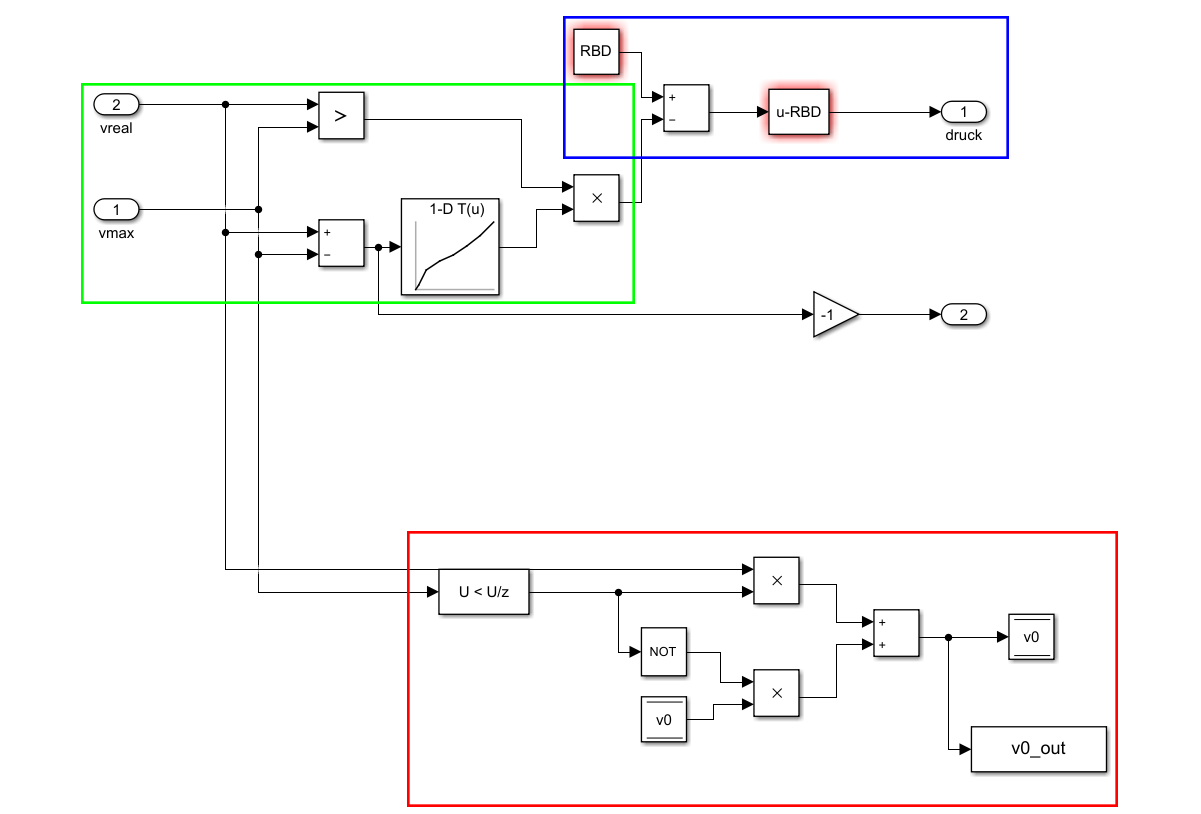
\includegraphics[width=\linewidth]{./pic/expandedmodel_pressure}
	\caption{Expanded model - Pressure Calculation}
	\label{fig:expandedmodel_pressure}
\end{figure}

\par\noindent
Depicted above is the system which determines braking pressure to apply. It calculates vdiff by subtracting vmax from vreal, which is then fed into a one-dimensional lookup table. The table is a sampled representation of a function with fixed breakpoints, mapping one function value to each breakpoint, like so \[
H(n) =
\begin{cases}
0.1 & \text{if $n=1$} \\
0.7 & \text{if $n=15$} \\
0.8 & \text{if $n=20$} \\
\text{..}
\end{cases}
\]

\par\noindent
where n are the breakpoints of vdiff. Since the pressure should only be applied if vreal is greater than vmax, the ultimate result follows the logic of the following equation \[
	f(n) = H(n) * (\text{vreal $>$ vmax})
\]

\par\noindent
where vreal $>$ vmax is either 1 or 0.

\section{Further Expansion}
\label{sec:FurtherExpansion}